\documentclass[paper]{ieicej}
%\documentclass[invited]{ieicej}% 招待論文
%\documentclass[survey]{ieicej}% サーベイ論文
%\documentclass[comment]{ieicej}% 解説論文
%\usepackage[dvips]{graphicx}
\usepackage[dvipdfmx]{graphicx,xcolor}
\usepackage[fleqn]{amsmath}
\usepackage{newtxtext}% 英数字フォントの設定を変更しないでください
\usepackage[varg]{newtxmath}% % 英数字フォントの設定を変更しないでください
\usepackage{latexsym}
%%図を二個横に並べるときに使用
\usepackage[hang,small,bf]{caption}
\usepackage[subrefformat=parens]{subcaption}


\setcounter{page}{1}

\jtitle{VAEを用いた画像圧縮,異常検知,\\(題名もうちょっと良いのないかな)}
%\etitle{imamura yuki}

\authorlist{%
\authorentry[imamura.yuuki475@mail.kyutech.jp]{今村 優希}{Yuki Imamura}{kyutech}
\authorentry[kawasaki.taiga000@mail.kyutech.jp]{川崎 大雅}{Taiga Kawasaki}{kyutech}
% \authorentry[メールアドレス]{和文著者名}{英文著者名}{所属ラベル}
}
\affiliate[kyutech]{九州工業大学情報工学部 情報・通信工学科 3年\\ 福岡県飯塚市川津680-4}
  {Kyushu Institute of Technology, School of Computer Science and System Engineering, Department of Computer Science and Networks}
%\affiliate[所属ラベル]{和文勤務先\\ 連絡先住所}{英文勤務先\\ 英文連絡先住所}
\jalcdoi{???????????}% ← このままにしておいてください

\begin{document}
\begin{abstract}
%和文あらまし 500字以内
あああああああああああああああああああああああああああああああああああああ
あああああああああああああああああああああああああああああああああああああ
あああああああああああああああああああああああああああああああああああああ
あああああああああああああああああああああああああああああああああああああ
あああああああああああああああああああああああああああああああああああああ
あああああああああああああああああああああああああああああああああああああ
あああああああああああああああああああああああああああああああああああああ
あああああああああああああああああああああああああああああ(大体300文字)
\end{abstract}
\begin{keyword}
%和文キーワード 4〜5語
VAE, FPGA, エッジコンピューティング
\end{keyword}
%\begin{eabstract}
%英文アブストラクト 100 words
%test
%\end{eabstract}
%\begin{ekeyword}
%英文キーワード
%VAE, FPGA, edge computing
%\end{ekeyword}
\maketitle

\section{はじめに}
近年,無線通信技術は飛躍的に向上しており,5G通信の普及が進んでいる.
5Gは従来の4Gなど通信規格と異なり,「高速大容量」「低遅延」「多数同時接続」の3つの特徴を備えており,その中でも「低遅延」と「多数同時接続」は新たな通信環境を構築する上で重要な軸となっている\cite{5g}.

従来の4G通信は,人が使用するスマートフォンや携帯に焦点を当てていた.
しかし,5Gでは車両,ドローン,センサなどのIoT機器が大量にネットワークに接続されることを前提としている.

このような環境においては,従来のクラウド中心の処理方式では,トラヒック増加による遅延や負荷集中が生じる可能性があり,5Gの利点を十分に発揮できない問題がある.
また,今現在のIT業界ではクラウドが主流で,処理の多くを一つ(もしくは複数の)コンピュータで行うという構造である.
多くの端末から取得したデータをクラウドのみで処理を行うのはある程度限界があり,またトラヒック量が増加して,5Gのメリットを享受できないという問題が発生すると考えられる.

このような課題を解決するため,エッジコンピューティングという技術が近年注目され始めている.
エッジコンピューティングとは,従来はクラウドで行っていた処理の一部を,ユーザ端末(スマートフォンやIoT機器)の近い位置である基地局やその至近に設置されているサーバなどでデータ処理を行う技術である\cite{edge-com}.
この技術を用いることでクラウドにかかる処理をエッジコンピューティングで分散することが可能で,通信のトラヒック量,5Gの特徴のひとつである「低遅延」に貢献することも可能である.

\begin{figure}[tb]
  \begin{center}
    \includegraphics[width=0.98\columnwidth]{figures/Intr_1.png}
  \end{center}
  \caption{エッジコンピューティングのイメージと\\今回のシステムの作成部分}
  \label{fig:1-1}
\end{figure}

そこで,エッジコンピューティングの実現をVAEとFPGAを用いて実現することを考えた.
(本文を書きながら続きを記述予定)

\section{方法}
\subsection{実行環境}
今回の設計において使用したツール及びそのバージョンを表\ref{tb:1}で示す.


\begin{table}[tb]
  \centering
  \caption{使用したツール}
  \small
  \begin{tabular}{|c|c|} \hline
    用途 & 使用ツール \\ \hline \hline
    VAEシミュレーション用 & MATLAB 2024b \\ \hline
    ハードウェアシミュレーション & MATLAB/Simulink 2022a\\ \hline
    HDLコード生成 & HDL Coder \\ \hline
    FPGA設計ソフトウェア & Vivado 2022.1\\ \hline
    ハードウェアアクセラレーション & Vitis xxxx \\ \hline
    評価ボード & DIGILENT製 ZYNQ-7010 \\ \hline
  \end{tabular}
  \label{tb:1}
\end{table}


\subsection{システム構造}
今回のVAEを搭載したシステムでは,以下2つの機能を搭載した.
\begin{itemize}
  \item[1] 画像圧縮\\
  VAEの特徴のひとつである次元圧縮能力を画像に応用する.
  \item[2] 異常検知\\
  もう一つの特徴である異常検知を,元画像と生成画像とを比較して行う.  
\end{itemize}

全体の構想について解説する.
今回使用する画像は,簡単化のためにグレースケール化したものを使用する.
また,JPEGのようにブロックに分割して,それぞれのブロック毎に処理を行う.
ブロックサイズは$16\times16$に設定した.

画像圧縮や異常検知の判定は,元画像と圧縮後の画像との比較をPSNRを用いて行う.
PSNRが設定した閾値以上だった場合は精度良く圧縮ができるているので圧縮した潜在空間の値を送信する.
それ以下だった場合は異常として通知を行う.

上記の機能を実現するために,VAEの構造を\ref{2.2.3}で説明する.
また,FPGAの構造の詳細を\ref{2.2.4}にて説明し,最後にSoC FPGAの構造を\ref{2.2.5}にて説明する.

\subsubsection{VAE構造}\label{2.2.3}
VAEの構造の概略を図\ref{fig:2-2-2-1}に示す.
$16×16$の画像を使用することから,入力256次元,出力256次元で設計を行った.
潜在空間の次元は,次元圧縮と異常検知という目的を両立させるために,16次元で設計を行った.
エンコーダ部分の活性化関数に関しては,平均ではReLU関数を使用し,分散ではソフトプラス関数を使用している.
また,デコーダ部分ではシグモイド関数を利用している.
\begin{align}
  f(x) &= x &: ReLU関数\\
  f(x) &= \log(1+e^x) &: Softplus関数 \label{sq:2}\\
  f(x) &= \dfrac{1}{1+e^{-x}} &: Sigmoid関数 \label{sq:3}
\end{align}

また,VAEの学習方法を図\ref{fig:2-2-2-2}に示す.
まず,道路のみが映った画像を用意する.
その画像に対して,道路のみ映った部分だけで$16\times16$のブロックにする.
そのブロックらを教師データとし,VAEを学習させる.
今回のシステムでは,MATLABでVAEの学習のみ行い,そこから出力された重みやパラメータを使用してLSI設計を行った.
学習の条件を表\ref{tb:2}にまとめた.

\begin{table}[b]
  \centering
  \caption{学習条件}
  \small
  \begin{tabular}{|c|c|} \hline
    epoch & 10000 \\ \hline
    eta & 0.0005 \\ \hline
    Layer2(潜在空間の数) & 16 \\ \hline
  \end{tabular}
  \label{tb:2}
\end{table}


% VAEの構造図
\begin{figure}[tb]
  \begin{center}
    %Created by Kawasaki, Edited by Imamura
    \includegraphics[width=0.98\columnwidth]{figures/VAE_1.bmp}
  \end{center}
  \caption{今回のVAEの構造}
  \label{fig:2-2-2-1}
\end{figure}

\begin{figure}[tb]
  \begin{center}
    \includegraphics[width=0.98\columnwidth]{figures/VAE_2.bmp}
  \end{center}
  \caption{VAE学習方法}
  \label{fig:2-2-2-2}
\end{figure}

\subsubsection{FPGA構造}\label{2.2.4}
使用したボードは,DIGILENT製のZYNQ-7010である.
今回の設計では,入力が34,出力が2の演算を行う.

入力データとして,$X$,$w2$,$b$を使用する.
$X$と$w2$は16個,$b$は2個である.
赤色の枠で囲われているユニットは,
\begin{align}
  Output_1 = X_1 \times w2_1
\end{align}
のような,入力と重みのパラメータを乗算する演算を行っている.
その演算ユニットを16個用意したものが,青色の枠線で囲われているユニットである.
青色のユニットでは,最終的に以下の計算を行っている.
\begin{align}
  Z_{21} = \sum_{i = 0}^{16} X_j \times W_{2j} + b2_1
\end{align}
そのユニットを2つ用意することで,出力を2つ得られるように設計した.

当初は入力256,出力256の演算をFPGAに載せたかったが,容量に限界があった.
したがって,今回設計した$256\times16\times256$のVAEに切りの良い数字を使った,$X$の入力が16になるように設計を行った.

FPGAに実装した後の評価を表\ref{tb:3}に示す.

\begin{table}[tb]
  \centering
  \caption{FPGAのリソース利用率}
  \small
  \begin{tabular}{|c|c|c|c|} \hline
    Resorce & Utilization & Available & Utilizatio[\%]\\ \hline
    LUT & 3301 & 17600 & 18.76 \\ \hline
    LUTRAM & 62 & 6000 & 1.03 \\ \hline
    FF & 3297 & 35200 & 9.37 \\ \hline
    DSP & 64 & 80 & 80.0 \\ \hline
    IO & 12 & 100 & 12.0 \\ \hline
    BUFG & 1 & 32 & 3.13 \\ \hline
  \end{tabular}
  \label{tb:3}
\end{table}

% FPGA内の構造図
% エンコーダの中身
\begin{figure}[tb]
  \begin{center}
    %入力画像はPNG
    %created by Imamura
    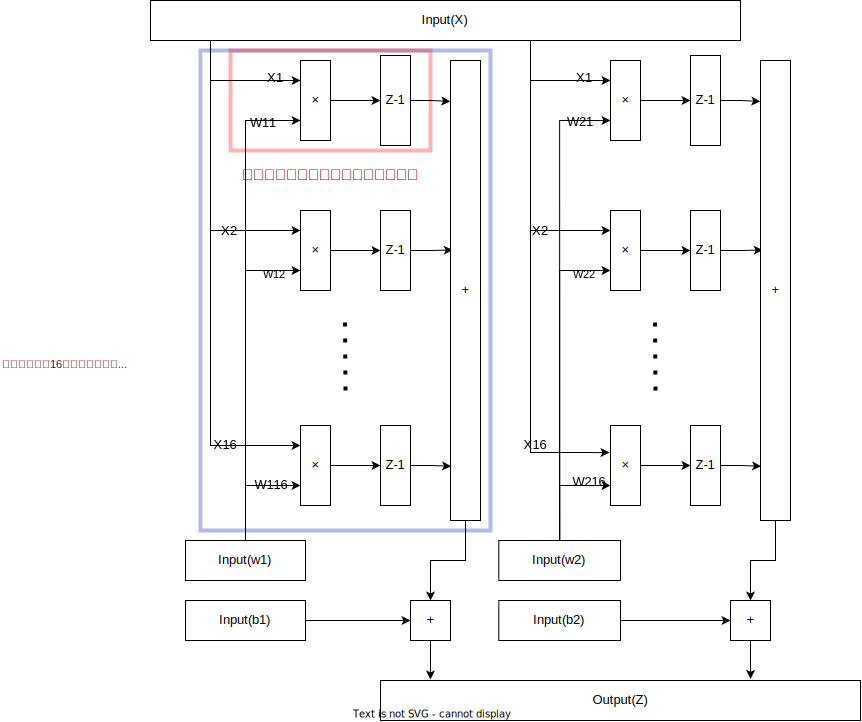
\includegraphics[width=0.98\columnwidth]{figures/FPGA_1.png}
  \end{center}
  \caption{FPGAの構造}
  \label{fig:2-2-3-1}
\end{figure}

\subsubsection{SoC FPGAの構造}\label{2.2.5}
SoC FPGAのシステム構造の概要を図\ref{fig:2-2-4-1}にて示す.
Processing Systemユニットがバスを通って様々な処理を行う.

次に,SoC FPGAの処理の概要を図\ref{fig:2-2-4-2}にて示す.
SDカードに格納されているVAEの学習重みや画像データをCPUが読み取る.
その後,作成したFPGAに従って入力データの処理を行い,FPGAにそのデータを送信する.
FPGAはデータが格納されると同時に実行し,出力結果を保存する.
その出力結果をCPUが読み取りに行き,出力データを処理する.
それらの処理を繰り返し行う.

今回のVAEが$256\times16\times256$であり,\ref{2.2.4}で作成したFPGAの構造が$16\times2$である.
設計したFPGAでエンコーダを計算する際は,一つの出力で$z^2_{mean}$を,もう一つの出力で$z^2_{var}$を計算させる.
1つの潜在空間を計算させるためには,FPGAを16回使用する必要がある.
その潜在空間が16個あるので,FPGAは合計で$16\times16=256$回稼働する.
デコーダ部分を計算する際は,FPGAを一回稼働させるだけで,3層目の出力を2つ得られる.
したがって,デコーダでは128回FPGAを稼働させる.
このような制御をCPUで作成した.

% SoC構造図
\begin{figure}[tb]
  \begin{center}
    %created by screenshot
    \includegraphics[width=0.98\columnwidth]{figures/SoC_1.png}
  \end{center}
  \caption{SoC FPGAの構成図}
  \label{fig:2-2-4-1}
\end{figure}

\begin{figure}[tb]
  \begin{center}
    \includegraphics[width=0.98\columnwidth]{figures/SoC_2.png}
  \end{center}
  \caption{SoC FPGAの処理概要}
  \label{fig:2-2-4-2}
\end{figure}

\subsection{実験方法}
今回は,図\ref{fig:3-1-1}のような車載カメラから取得した画像をイメージとしたものを利用する.
また,プロトタイプの作成として,画像の一部のブロックに対してVAEを活用した画像圧縮,異常検知を行うようにした.
一部のブロックの選出については図\ref{fig:3-1-2}のように設定しており,車がこれから通過するであろう部分を判定するように設定した.
図\ref{fig:3-1-2}における赤枠の大きさは,$16\times16$である.

実際に,図のようなテスト画像を用意した.
実際にVAEで判定させるものは図の白黒画像である.
この図は,道路に落下物が落ちていることを想定しており,今回のシステムにおける異常検知の実施を行う.

\begin{figure}[tb]
  \begin{minipage}[]{0.49\columnwidth}
    \centering
    \includegraphics[width=0.9\columnwidth]{figures/Ex_re_2.png}
    \subcaption{車載カメラからの\\イメージ図}
    \label{fig:3-1-2}
  \end{minipage}
  \begin{minipage}[]{0.49\linewidth}
    \centering
    \includegraphics[width=0.9\columnwidth]{figures/Ex_re_1.png}
    \subcaption{評価対象例\\ 赤枠の部分をVAEにて評価する}
    \label{fig:3-1-3}
  \end{minipage}
  \caption{今回のシステムで評価する方法\\これいらんかもな}
  \label{fig:3-1-1}
\end{figure}

\begin{figure}[tb]
  \begin{minipage}[]{0.49\columnwidth}
    \centering
    \includegraphics[width=0.9\columnwidth]{figures/Ex_re3.png}
    \subcaption{評価する画像}
    \label{fig:3-1-5}
  \end{minipage}
  \begin{minipage}[]{0.49\linewidth}
    \centering
    \includegraphics[width=0.9\columnwidth]{figures/Ex_re4.png}
    \subcaption{評価画像をグレーに変更}
    \label{fig:3-1-6}
  \end{minipage}
  \caption{今回テストする評価画像}
  \label{fig:3-1-4}
\end{figure}

\section{実験と考察}
\subsection{実験方法}

\subsection{実験結果}
えーまだ,このFPGAを使用したメインプログラムが作成できていないので記述できません...

\subsection{考察}
出力された画像とシミュレーションした画像の比較を行う.

\section{結論と今後の展望}
結論として,

今回は,エッジコンピューティングを意識し,VAEをFPGAを用いて実装を行った.
5Gが浸透していき,様々なIoT機器がネットに繋がるようになると考えられる.
その際に,いかに効率よく伝送し,早く制御を行うかが重要になってくると思う.
今後,VAEやFPGAが自動運転を含む様々な分野で応用されていくと考えられ,今回の開発はこれからの発展の初期的な内容のものであると考えることができる.

使用した評価ボートに載せることのできる回路に制限があり,思うような回路を作成することができなかった.
しかし,16入力-2出力の回路を作成し,この回路でVAEのエンコードもデコードもできるようプログラムできたことは良かったと感じる.
これからもFPGAを用いた開発を行っていきたいし,高位合成等のFPGAを開発するための技術も日々進化しているので,様々なことに挑戦していきたい.

\ack
今回のシステム構築に対して,様々な支援を頂いた方々に感謝する.
%\bibliographystyle{sieicej}
%\bibliography{myrefs}
\begin{thebibliography}{99}% 文献数が10未満の時 {9}
\bibitem{5g} 
森川博之, 5G次世代移動通信規格の可能性, 岩波書店, 
\bibitem{edge-com} 
田中裕也, 高橋紀之, 河村龍太郎, "IoT時代を拓くエッジコンピューティングの研究開発", NTT技法ジャーナル, vol.27, no.8, pp.59-63, 2015.
\end{thebibliography}

\end{document}
